\chapter{Dịch máy bằng mô hình học LSTM-Attention}
\ifpdf
    \graphicspath{{Chapter3/Chapter3Figs/PNG/}{Chapter3/Chapter3Figs/PDF/}{Chapter3/Chapter3Figs/}}
\else
    \graphicspath{{Chapter3/Chapter3Figs/EPS/}{Chapter3/Chapter3Figs/}}
\fi
\label{chap_3}
\begin{quote}
\textit{Chương này trình bày về mô hình học LSTM-Attention cho bài toán Dịch máy dựa trên bài báo "Effective Approaches to Attention-based Neural Machine Translation" \cite{attentionThangLuong2015} được công bố tại hội nghị EMNLP của nhóm tác giả thuộc Đại học Stanford gồm Minh-Thang Luong, Hieu Pham, Christopher D. Manning. Chúng tôi trình bày về việc tổ chức các LSTM theo kiến trúc Bộ mã hóa - Bộ giải mã cùng với sử dụng các phiên bản của cơ chế Attention, đồng thời giải thích chúng dựa trên cơ sở Toán học. Cụ thể:
\begin{itemize}
	\item LSTM: chúng tôi tổ chức các theo kiến trúc Bộ mã hóa - Bộ giải mã để tránh được ràng buộc về số lượng từ ở ngôn ngữ nguồn và ngôn ngữ đích khi dùng một LSTM để dịch.
	\item Attention: chúng tôi tìm hiểu sự hạn chế hiện có của kiến trúc Bộ mã hóa - Bộ giải mã khi thực hiện dịch những câu dài. Từ đó, cơ chế Attention được sử dụng để giải quyết hạn chế đó bằng cách sử dụng thêm các trạng thái ẩn của bộ mã hóa trong quá trình giải mã.
	\begin{itemize}
		\item Toàn cục: phiên bản này sử dụng tất cả trạng thái ẩn trong bộ mã hóa trong quá trình giải mã.
		\item Cục bộ: phiên bản này chỉ sử dụng một số trạng thái ẩn trong bộ mã hóa trong quá trình giải mã.
	\end{itemize}
\end{itemize}}
\end{quote}
\section{Mô hình học LSTM cho bài toán Dịch máy}
Với những kiến thức về mô hình LSTM mà đã được trình bày ở chương trước, dùng một mô hình LSTM hoàn toàn có thể áp dụng cho việc giải quyết bài toán Dịch máy. Với đầu vào tại mỗi bước thời gian là một từ ở trong câu nguồn và đầu ra là một từ tương ứng trong ngôn ngữ đích. Tuy nhiên, do bản thân của mô hình LSTM, khi sử dụng một mô hình LSTM áp dụng cho bài toán Dịch máy thì phải chịu một số hạn chế. Một trong những hạn chế lớn nhất chính là ràng buộc chiều dài của câu đầu vào (câu ở ngôn ngữ nguồn) phải bằng chiều dài của câu đầu ra (câu ở ngôn ngữ đích). Hơn nữa, đối với những ngôn ngữ có trật tự từ khác nhau như tiếng Anh (chủ ngữ-vị ngữ-tân ngữ) và tiếng Nhật (chủ ngữ-tân ngữ-vị ngữ) thì với một LSTM mô hình không thể dịch tốt được.

Để giải quyết những hạn chế của đó, nhóm tác giả Sutskever, 2014 \cite{Seq2Seq2014} đã đề xuất một kiến trúc tên gọi là \textit{Chuỗi tới Chuỗi (Sequence to Sequence - Seq2Seq)}. Tuy nhiên, mọi người thường gọi kiến trúc này là kiến trúc Bộ mã hóa - Bộ giải mã (Encoder-Decoder). Trong khóa luận này, chúng tôi tìm hiểu và dùng kiến trúc này để giải quyết bài toán Dịch máy và gọi nó là Bộ mã hóa - Bộ giải mã.

Kiến trúc Bộ mã hóa  -Bộ giải mã như tên gọi, gồm có hai bộ phận chính là bộ mã hóa và bộ giải mã. Mỗi một bộ phận sẽ là một mô hình học được lựa chọn sao cho phù hợp với bài toán và có thể hoạt động tốt với nhau. Đối với bài toán Dịch máy và trong phạm vi khóa luận này, mỗi bộ phận sẽ là một mạng nơ-ron hồi qui, cụ thể là một LSTM. Các LSTM trong kiến trúc sẽ được sắp xếp một cách hợp lí dựa trên những đặc tính của chúng sao cho phù hợp với bài toán Dịch máy.

\begin{figure}
	\centering
	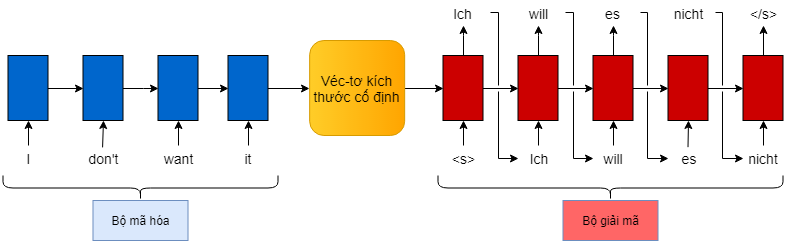
\includegraphics[width=1.0\textwidth]{Encoder-Decoder_2}
	\caption[Minh họa kiến trúc Bộ mã hóa - Bộ giải mã được sử dụng trong khóa luận.]{Minh họa kiến trúc Bộ mã hóa - Bộ giải mã được sử dụng trong khóa luận. Kiến trúc có hai bộ phận. Trong đó, bộ mã hóa là một bi-LSTM có nhiệm vụ nhận câu nguồn làm đầu vào và xuất ra một véc-tơ có kích thước cố định chứa thông tin cần thiết để dịch của toàn bộ câu nguồn. Bộ giải mã là một uni-LSTM có đầu vào là véc-tơ có kích thước cố định của bộ mã hóa và đầu ra là câu đích.}
	\label{fig_Encoder-Decoder}
\end{figure}

Hình \ref{fig_Encoder-Decoder} minh họa kiến trúc Bộ mã hóa - Bộ giải mã được sử dụng trong khóa luận để giải quyết bài toán Dịch máy. Chúng tôi sẽ trình bày cụ thể về cách hoạt động của hai bộ phận này trong các phần tiếp theo.

\subsection{Bộ mã hóa}
Bộ mã hóa là một bi-LSTM (LSTM hai chiều). Bi-LSTM này nhận đầu vào là một câu ở ngôn ngữ nguồn $\bm{x} = \{x_1, ..., x_S\}$ với S là chiều dài, $x_1,...x_S$ là các từ trong câu. Đầu ra là một véc-tơ có kích thước cố định. Véc-tơ này chứa các thông tin cần thiết để tiến hành dịch sang câu ở ngôn ngữ đích. Nhiệm vụ của bộ mã hóa (bi-LSTM) là thực hiện mã hóa toàn bộ câu nguồn thành véc-tơ có chứa các thông tin hữu ích. Véc-tơ kích thước cố định này rất quan trọng, nó là tiền đề để việc dịch sang câu đích đạt chất lượng tốt.

Ở đây, véc-tơ trạng thái ẩn $\bm{h}_S$ (trạng thái ẩn cuối cùng trong bi-LSTM) được sử dụng làm véc-tơ có kích thước cố định. Lí do bởi vì trong bi-LSTM, trạng thái ẩn của một từ thứ $t$ (tại bước thời gian $t$) chứa những thông tin, mỗi quan hệ giữa từ này và những từ lân cận. Hơn nữa, nó còn chứa thông tin của toàn bộ những từ ở đầu câu cho tới từ thứ $t$. Vậy nên trạng thái ẩn của từ cuối cùng của câu sẽ chứa đựng thông tin của toàn bộ những từ trong câu. Và điều đó phù hợp với ý tưởng của véc-tơ có kích thước cố định của bộ mã hóa. Điểm đặc biệt của bi-LSTM trong bộ mã hóa này so với các LSTM thông thường khác là do chúng tôi chỉ sử dụng véc-tơ trạng thái ẩn cuối cùng làm đầu ra của bộ mã hóa, vì vậy bi-LSTM này tại tất cả bước thời gian đều không xuất ra bất kỳ đầu ra nào. Hình \ref{fig_Encoder-Decoder} minh họa loại bi-LSTM được sử dụng cho bộ mã hóa trong khóa luận (bên trái). Tại mỗi bước thời gian, bi-LSTM nhận một từ ở câu ngôn ngữ nguồn và thực hiện cập nhật trạng thái ẩn cho đến hết câu.

Một cách tổng quát, bộ mã hóa là một mô hình mà nó mã hóa toàn bộ một đầu vào bất kì thành một véc-tơ bất kì mà véc-tơ đó chứa đầy đủ những thông tin cần thiết để thực hiện các công việc sau này. Trong một số công trình, họ sử dụng thêm một số phép biến đổi trên trạng thái ẩn cuối cùng của bi-LSTM để tạo ra một véc-tơ đầu ra phù hợp với mục đích của họ. Đối với bài toán như Phát sinh câu miêu tả cho ảnh, đầu ra của bộ mã hóa thường là một véc-tơ kích thước cố định chứa đặc trưng hữu ích của toàn bộ bức ảnh. Còn đối với bài toán Tóm tắt văn bản, đầu ra của bộ mã hóa là một véc-tơ chứa toàn bộ thông tin cần thiết dùng cho việc tóm tắt của văn bản đầu vào.

\subsection{Bộ giải mã}
Bộ giải mã là một uni-LSTM (LSTM một chiều). Uni-LSTM này nhận đầu vào là một véc-tơ kích thước cố định chứa thông tin cần thiết của câu cần dịch. Véc-tơ này là véc-tơ kích thước cố định từ đầu ra của bộ mã hóa. Đầu ra của bộ giải mã là câu đã được dịch sang ngôn ngữ đích $\bm{y} = \{y_1, ..., y_{S^{'}}\}$ với $S^{'}$ là chiều dài của câu đích, $y_1, ...,y_{S^{'}}$ là các từ trong câu đích.
Lí do chúng tôi sử dụng uni-LSTM mà không phải là bi-LSTM bởi vì trong quá trình giải mã (dịch) mô hình chỉ biết có được những từ đã được dịch ở trước đó (thông tin trong quá khứ) mà không biết được những từ đằng sau (thông tin trong tương lai) (vì những từ phía sau chưa được dịch). Do đó, việc sử dụng lợi thế của bi-LSTM trong bộ giải mã là không thể và có thể gây ảnh hưởng tới chất lượng dịch của mô hình. Hình \ref{fig_Encoder-Decoder} minh họa loại uni-LSTM được sử dụng cho bộ giải mã trong khóa luận này (bên phải). Ở bước thời gian đầu tiên, uni-LSTM nhận đầu vào là kí tự bắt đầu câu \textit{<s>} và dự đoán từ đầu tiên của câu đích. Tại mỗi bước thời gian tiếp theo, bi-LSTM này nhận đầu vào là một từ đã dự đoán ở bước thời gian trước và dự đoán từ tiếp theo cho đến khi bi-LSTM dự đoán ra kí hiệu kết thúc câu \textit{</s>}.

Một điều đáng lưu ý trong việc huấn luyện uni-LSTM trong bộ giải mã đó là đầu vào của uni-LSTM trong mỗi bước thời gian $t$. Hình \ref{fig_Encoder-Decoder} minh họa bộ giải mã trong quá trình suy diễn (là quá trình mà sau khi mô hình đã huấn luyện xong được mang đi dịch). Từ được dự đoán ở bước thời gian $t-1$ sẽ là đầu vào của uni-LSTM ở bước thời gian $t$. Tuy nhiên, việc như vậy sẽ là hạn chế lớn nếu sử dụng nó trong quá trình huấn luyện. Lí do bởi vì tại mỗi bước thời gian $t$, khi thực hiện dự đoán từ đích tiếp theo, mô hình sẽ dựa vào những từ ở phía trước để dự đoán, rồi sau đó sẽ tính độ lỗi dựa trên từ đúng được cung cấp trong dữ liệu huấn luyện. Do vậy, có sự phụ thuộc giữa từ hiện tại và các từ phía trước nó trong quá trình dịch. Việc dự đoán tại bước thời gian $t$ có tốt hay không còn cần phải xem những từ đã được dự đoán ở phía trước có tốt hay không nữa. Nếu những từ ban đầu dự đoán không tốt, tất cả những được dự đoán ở phía sau sẽ càng kém hơn. Để mô hình có thể học được cách dịch một câu dài với quá trình huấn luyện như trên thì phải tốn nhiều thời gian và công sức tinh chỉnh mô hình. Vì vậy, chúng tôi đã tìm hiểu và sử dụng phương pháp huấn luyện mạng nơ-ron hồi quy hiệu quả là \textit{teacher forcing} (tạm dịch là hướng dẫn của giáo viên). Phương pháp này đơn giản là tại mỗi bước thời gian $t$, từ đúng tại $t-1$ sẽ làm đầu vào của mạng tại bước thời gian $t$. Tức là mô hình tại mỗi bước thời gian $t$ đều nhận được đầu vào đúng bất kể kết quả dự đoán của bước thời gian trước $t-1$. Hình \ref{fig_Teacher-forcing} minh họa phương pháp teacher forcing. Với phương pháp này, mô hình hội tụ nhanh hơn so với việc sử dụng cách huấn luyện ở trên. Bởi vì khi dịch những câu dài, lúc dự đoán một từ thì không phải phụ thuộc hoàn toàn vào những từ đã được dự đoán trước đó mà dựa vào những từ đúng đã được cung cấp. Khi thực hiện quá trình suy diễn thì hiển nhiên sẽ phải dùng kết quả của những lần dự đoán phía trước để dự đoán từ tiếp theo hiện tại. 

\begin{figure}
	\centering
	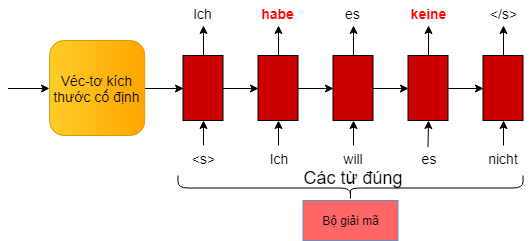
\includegraphics[width=0.7\textwidth]{Teacher-forcing.png}
	\caption[Minh họa phương pháp teacher forcing.]{Minh họa phương pháp teacher forcing. Đầu vào tại các bước thời gian là các từ đúng dù ở bước thời gian trước mô hình có đưa ra dự đoán sai.}
	\label{fig_Teacher-forcing}
\end{figure}

Trong quá trình giải mã, bộ giải mã thực hiện dự đoán từ tiếp theo dựa trên những từ đã biết trước đó: $p(y_t | y_{<t}, \bm{x})$. Việc quyết định xem chọn từ nào sẽ là từ tiếp theo dựa trên những xác suất $p_t$ trên tất cả các từ có trong bộ từ vựng $V$ mà đã tính được là một chiến lược quan trọng trong quá trình giải mã. Với chiến lược đúng đắn, mô hình sẽ cải thiện được chất lượng của đầu ra mà không phải thay đổi bộ tham số của mô hình thông qua các cách như huấn luyện mô hình.

Cách đơn giản nhất để quyết định xem nên chọn từ nào từ phân phối xác suất trên bộ từ vựng $P(\bm{y} | y_{<t}, \bm{x}\})$ là chọn ra từ nào có xác suất cao nhất:
\begin{equation}
\hat{y} = \operatorname*{argmax}_{y_t \in V} (p(y_t | y_{<t}, \bm{x}))
\end{equation}
Cách mà lựa chọn những từ theo tiêu chí có xác suất cao nhất này được gọi là \textit{thuật toán tìm kiếm tham lam} (\textit{greedy search algorithm}). Tuy nhiên, cách này trong thực tế cho ra kết quả không thực sự tốt. Để làm rõ hơn về sự hạn chế của thuật toán tìm kiếm tham lam trong thực tế, chúng tôi lấy một ví dụ trong quá trình dịch từ một câu tiếng Đức "Ich schwimme am nächsten Wochenende" sang tiếng Anh như sau: "I am swimming at the next weekend" hoặc "I am going to be swimming playing at the next weekend". Dễ thấy, câu dịch đầu tiên "I am swimming at the next weekend" là câu dịch tốt hơn vì nó ngắn mà vẫn đảm bảo đầy đủ ý của câu. Câu dịch thứ hai "I am going to be swimming playing at the next weekend" mặc dù vẫn đảm bảo ý nghĩa của câu nhưng lại dài hơn. Vấn đề của tìm kiếm tham lam phát sinh từ đây. Giả sử, mô hình thực hiện quá trình giải mã và đã dịch được hai từ đầu tiên "I am". Để đơn giản, chúng tôi giả định mô hình đang trong quá trình kiểm thử nên không sử dụng teacher forcing. Khi đó, xác suất của từ tiếp theo khi cho trước hai từ "I am":
\begin{equation*}
\hat{y_t} = \operatorname*{argmax}_{y_t \in V} p(y_t | I, am, \bm{x})
\end{equation*}
Trong tiếng Anh, dễ nhận thấy rằng tần số xuất hiện của "I am going" lớn hơn của "I am swimming", do đó rất có khả năng bộ giải mã sẽ tính toán ra được rằng $p(going | I, am) > p(swimming|I, am)$ và dẫn tới câu kết quả thứ hai "I am going to be swimming at the next weekend" mà không phải là câu dịch tốt hơn. Ví dụ chúng tôi vừa trình bày thể hiện rằng với thuật toán tìm kiếm tham lam, kết quả mà bộ giải mã đưa ra sẽ bị ảnh hưởng rất nhiều bởi những từ có tần số xuất hiện lớn trong tập dữ liệu huấn luyện. Do đó, mô hình sẽ thường có xu hướng cho ra những câu dịch mà trong đó những từ phổ biến như the, a, an, and, of, to, v.v... và tạo ra những câu dịch không thực tế, không phù hợp ngữ pháp, gây giảm chất lượng dịch của mô hình đi đáng kể. Thực chất, vấn đề của tìm kiếm tham lam là chỉ lựa chọn một từ duy nhất mà có xác suất có điều kiện $p(y_t | y_{<t}, \bm{x})$ lớn nhất và chỉ xét một \textit{câu giả thuyết (hypothesis)} duy nhất trong quá trình giải mã. Khi bộ giải mã dịch một câu, sẽ có nhiều câu ứng viên, mỗi câu ứng viên này chúng tôi gọi là một câu giả thuyết.

Khi thực hiện công việc dịch, mọi người nhìn vào câu nguồn và dịch ra từng từ ở câu đích. Tuy nhiên, ngôn ngữ tự nhiên rất phức tạp, mỗi một ngôn ngữ sẽ có ngữ pháp, hành văn khác nhau cũng như mối quan hệ giữa các từ trong câu cũng sẽ có trật tự riêng nên khó có thể dịch nhanh chóng trong một lần. Do đó, sau khi dịch được một số lượng từ nhất định hay hết một ý, mọi người cần phải nhìn lại những từ đã dịch và chỉnh sửa lại sao cho câu văn trôi chảy, mạch lạc, ý nghĩa hoàn thiện hơn.

Từ hạn chế của tìm kiếm tham lam và quá trình dịch trong thực tế, để dịch câu tối ưu hơn, mô hình sẽ dùng sử dụng tất cả tổ hợp của các từ để xây dựng thành các câu giả thuyết và đánh giá xem câu nào là tốt nhất bằng xác suất của các câu giả thuyết đó thông qua mô hình ngôn ngữ, câu tối ưu $\bm{\hat{y}}$ được lựa chọn dựa trên biểu thức:
\begin{equation*}
\bm{\hat{y}} = \operatorname*{argmax}_{\bm{y}} p(\bm{y})
\end{equation*}
Tuy nhiên, với số lượng từ vựng lớn, ví dụ bộ từ vựng $V = 10000$ từ thì số lượng tổ hợp câu gải thuyết có thể có là $V^S$, với $S$ là số từ trong câu. Với cách này, mô hình có thể đảm bảo được rằng câu dịch ra là tối ưu dựa trên trạng thái mô hình hiện có nhưng chi phí tính toán rất lớn và lưu trữ rất lớn. Do vậy, việc mà có thể làm được hiện tại là tìm kiếm gần đúng trên không gian tổ hợp các câu giả thuyết đó. Thuật toán tìm kiếm gần đúng này được gọi là \textit{beam search} (tạm dịch: \textit{tìm kiếm theo chùm}).

Beam search về cơ bản có cách hoạt động giống tìm kiếm tham lam. Khác biệt ở đây là khi dự đoán, thay vì chỉ dùng một câu giả thuyết có xác suất lớn nhất thì beam search chọn $B$ câu giả thuyết có xác suất lớn nhất. $B$ là một siêu tham số chỉ kích thước của beam (chùm). Do beam search dùng $B$ câu giả thuyết, do đó để lựa chọn $B$ câu giả thuyết có xác suất lớn nhất thì cần phải tính xác suất của từng câu. Cách tính xác suất cho một câu giống như mô hình ngôn ngữ:
\begin{equation}
p(\bm{y}) = p(y_1, y_2, ..., y_{S} | \bm{x}) = p(y_1 | \bm{x}) p(y_2 | p_1, \bm{x})...p(y_{S} | y_1, y_2, ...,y_{S-1}, \bm{x})
\end{equation}
Để làm rõ hơn cách hoạt động của beam search, chúng tôi xét lại ví dụ dịch câu tiếng Đức "Ich schwimme am nächsten Wochenende" sang tiếng Anh. Trong ví dụ này chúng tôi lựa chọn $B = 3$. Bộ giải mã khởi tạo $B = 3$ câu giả thuyết rỗng (không có từ nào). Mô hình có bộ từ vựng $V = \{a,an,...,zoo\}$. Tại bước thời gian đầu, bộ giải mã nhận đầu vào là kí tự bắt đầu câu \textit{<s>}. Sau đó, đối với mỗi câu giả thuyết, bộ giải mã thực hiện dự đoán từ tiếp theo bằng cách tính xác suất có điều kiện dựa trên câu giả thuyết hiện tại, câu đầu vào và bộ từ vựng $V$: $p(y_1 | <s>, \bm{x}), \ y_1 \in V$. Xét tất cả các xác suất có điều kiện $p(y_1 | <s>, \bm{x})$ vừa tính được trên cả 3 câu giả thuyết, mô hình lựa chọn ra $B = 3$ câu có xác suất $p(y_1, <s> | \bm{x})$ cao nhất.
\begin{equation*}
p(y_1, <s> | \bm{x}) = p(y_1 | <s>, \bm{x}),\ y_1 \in V
\end{equation*}
Giả sử, các từ $y_1$ "I", "At", "The" làm xác suất $p(y_1, <s> | \bm{x})$ cao nhất và được mô hình lựa chọn làm 3 câu giả thuyết. Tiếp theo, mô hình tiếp tục dự đoán từ tiếp theo và tính các xác suất câu $p(y_2 | <s>, "I")$, $p(y_2 | <s>, "At")$, $p(y_2 | <s>, "The")$. Tiếp tục giả định rằng mô hình có 3 câu có xác suất cao nhất là "I am", "At the", "The next" (để đơn giản, chúng tôi không ghi lại kí tự bắt đầu câu \textit{<s>}) và mô hình chọn 3 câu này thành 3 câu giả thuyết. Mô hình lại tiếp tục dự đoán từ tiếp theo cho 3 câu giả thuyết hiện có và tính xác suất câu để tìm ra câu có xác suất cao nhất. Lần này xác suất 3 câu "I am swimming", "I am going", "The next weekend" là lớn nhất, tức là câu "The next" không còn được chọn là cách dịch phù hợp nữa và bị loại bỏ. Cứ lặp lại như vậy cho đến khi cả 3 câu đều đã dự đoán ra kí tự kết thúc câu \textit{</s>} hoặc đã đạt tới giới hạn chiều dài do người dùng đặt thì dừng. Bây giờ mô hình có được 3 câu giả thuyết "I am swimming at the next weekend", "I am going to be swimming at the next weekend" và "At the next weekend, I am swimming". Cuối cùng, mô hình tính được câu giả thuyết "I am swimming at the next weekend" có xác suất cao nhất. Vậy mô hình chọn "I am swimming at the next weekend" làm kết quả cuối cùng. Hình \ref{fig_beam-search} minh họa thuật toán beam search cho ví dụ vừa trình bày.
\begin{figure}
	\centering
	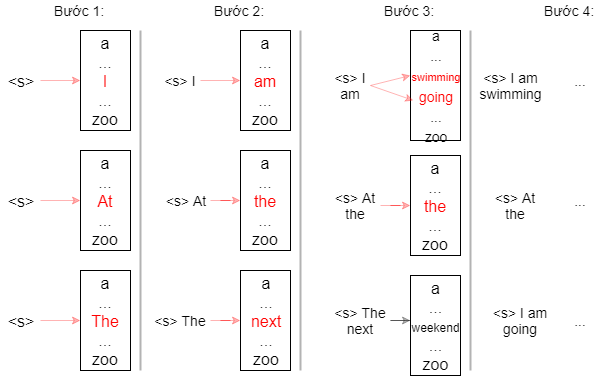
\includegraphics[width=0.9\textwidth]{beam-search.png}
	\caption[Minh họa thuật toán beam search.]{Minh họa thuật toán beam search.}
	\label{fig_beam-search}
\end{figure}
Về chi phí tính toán, trong ví dụ này, giả sử $V = 10000$, thì mô hình phải tính  $V \times B = 10000 \times 3 = 30000$ xác suất có điều kiện $p(y_t | y_{<t}, \bm{x})$  và phải tính $30000$ xác suất câu $p(\bm{y} | \bm{x})$ cho mỗi trường hợp vừa dự đoán nữa. Tổng cộng là $60000$. Tóm lại, chi phí tính toán của beam search so với tìm kiếm tham lam là gấp $2B$ lần.

Với ví dụ chúng tôi đã trình bày ở trên thể hiện rằng beam search giải quyết được hạn chế của thuật toán tìm kiếm tham lam và dịch ra được những câu tối ưu hơn. Tuy nhiên, vì beam search là thuật toán tìm kiếm gần đúng nên không thể đảm bảo rằng kết quả luôn là tối ưu như các thuật toán tìm kiếm chính xác Depth First Search, Bread First Search. Ưu điểm lớn nhất của beam search chính là nó khả thi trong thực tế nhờ tốc độ rất nhanh mà vẫn đảm bảo được đầu ra tốt. Việc lựa chọn kích thước của beam $B$ cũng rất quan trọng. Nếu chúng ta chọn $B = 1$, beam search trở thành thuật toán tìm kiếm tham lam. Với $B$ càng lớn thì có xu hướng cho ra kết quả tốt hơn, nhưng bù lại tốc độ và chi phí không gian lưu trữ tăng cao. Ngược lại, với $B$ nhỏ thì tốc độ nhanh, tiết kiệm chi phí không gian lưu trữ nhưng kết quả có xu hướng kém đi. Việc lựa chọn $B$ như thế nào phù thuộc vào từng hoàn cảnh. Trong Dịch máy, thường mọi người chỉ chọn $B = 5, 10, 15$. Trong một số ứng dụng, thậm chí $B = 1000$ tới $3000$. Cần lưu ý rằng không phải lúc nào kích thước beam $B$ càng lớn thì chất lượng dịch sẽ càng tốt mà còn phụ thuộc vào chất lượng của mô hình nữa. Cho nên, để có thể có được những câu dịch trôi chảy, chất lượng thì còn cần phải thực hiện phân tích kĩ càng hơn để xem là vấn đề nằm ở beam search hay là nằm ở mô hình.

Trong bài toán Dịch máy, beam search thường chỉ được sử dụng trong quá trình suy diễn. Bởi vì trong quá trình huấn luyện, mô hình sử dụng phương pháp teacher forcing có hiệu quả lớn hơn về mặt chi phí tính toán, tốc độ hội tụ cũng như dễ cài đặt.
\section{Mô hình học LSTM-Attention cho bài toán Dịch máy}
\subsection{Cơ chế Attention}
Ở phần trước, chúng tôi đã trình bày về kiến trúc Bộ mã hóa - Bộ giải mã cùng với những điểm mạnh của nó trong việc giải quyết bài toán Dịch máy. Tuy nhiên, kiến trúc này vẫn còn tồn tại hạn chế về việc dịch những câu dài do những thông tin được mã hóa của câu nguồn bị mất dần theo các bước thời gian về sau. Lí do mà vấn đề này tồn tại thực chất là bởi vì các mô hình LSTM được sử dụng trong bộ mã hóa và bộ giải mã. Bản thân mô hình LSTM chưa thật sự giải quyết hoàn toàn vấn đề "sự phụ thuộc dài hạn". Để có thể vẫn tận dụng được các mô hình LSTM mà vẫn nâng cao được chất lượng dịch, cơ chế Attention được sử dụng.

Trước khi đi vào cách hoạt động của cơ chế Attention, chúng tôi điểm qua một chút về nguồn cảm hứng và lịch sử của cơ chế này. Cơ chế Attention được lấy cảm hứng trên cách đặt sự chú ý khi quan sát sự vật, hiện tượng của thị giác con người. Khi con người quan sát một sự vật, hiện tượng nào đó bằng mắt, con người chỉ có thể tập trung vào một vùng nhất định trên sự vật, hiện tượng được quan sát để ghi nhận thông tin. Sau đó, khi cần ghi nhận thêm thông tin khác, con người sẽ di chuyển vùng tập trung của mắt sang vị trí khác trên vật thể, hiện tượng. Những vùng lân cận xung quanh vùng tập trung sẽ bị "mờ" hơn so với vùng tập trung. Cơ chế Attention đã được ứng dụng trong lĩnh vực Thị giác máy tính từ khá lâu \cite{attentionhistory2010} \cite{attentionhistory2011}. Vào những năm gần đây, cơ chế Attention được sử dụng cho các kiến trúc mạng nơ-ron hồi quy trên bài toán Dịch máy và đã đạt được những kết quả ấn tượng.

\begin{figure}
	\centering
	\includegraphics[width=0.8\textwidth]{Attention-3}
	\caption[Minh họa cơ chế Attention.]{Minh họa cơ chế Attention. Một tầng Attention được đặt ở trước bước dự đoán đầu ra của bộ giải mã. Bộ giải mã có thêm một số bước tính toán trước khi dự đoán từ tiếp theo ở câu đích. Bộ giải mã tính trọng số gióng hàng $\bm{a}_t$ cho một số trạng thái ẩn ở bộ mã hóa được lựa chọn. Sau đó tính véc-tơ ngữ cảnh $\bm{c}_t$ và nối véc-tơ này với trạng thái ẩn hiện tại của bộ giải mã thành véc-tơ attention $\bm{\tilde{h}}_t$. Cuối cùng mô hình dự đoán từ tiếp theo dựa trên véc-tơ attention vừa tính được.}
	\label{fig_Attention}
\end{figure}
Cơ chế Attention được sử dụng trong đề tài này là một cơ chế sử dụng thông tin trong các trạng thái ẩn của LSTM trong bộ mã hóa khi thực hiện quá trình giải mã. Cụ thể là:
\begin{itemize}
	\item Trong quá trình giải mã, trước khi dự đoán đầu ra, bộ giải mã "nhìn" vào các thông tin nằm trong các trạng thái ẩn của LSTM ở bộ mã hóa.
	\item Ở mỗi phần tử đầu ra tại bước thời gian $t$, bộ giải mã dựa vào trạng thái ẩn tại bước thời gian $t$ hiện tại và quyết định sử dụng các thông tin trong trạng thái ẩn ở bộ mã hóa như thế nào.
\end{itemize}
Hai phiên bản Toàn cục và Cục bộ mà trong khóa luận này chúng tôi trình bày là hai cách mà cơ chế Attention sử dụng các trạng thái ẩn của LSTM trong bộ mã hóa.
Để làm rõ hơn về ý tưởng của cơ chế Attention, dưới đây chúng tôi sẽ trình bày chi tiết về công thức tính toán của nó.
Attention sử dụng thêm một số đại lượng:
\begin{itemize}
	\item $\bm{a}_t$: véc-tơ trọng số gióng hàng. Gồm có các phần tử $a_{ts},\ s \in \{1, ..., S\}$, $\bm{a}_t$ được tính theo công thức dưới đây:
	\begin{equation}
	a_{ts} = \text{align}(\bm{h}_t, \bm{h}_s) = \frac{\exp\left(\text{score}(\bm{h}_t, \bm{h}_s)\right)}{\sum_{s^{'}}\exp\left(\text{score}(\bm{h}_t, \bm{h}_{s^{'}})\right)}
	\end{equation}
	$a_{ts}$ là một số thực nằm trong đoạn $[0;1]$ thể hiện mức độ mà trạng thái ẩn ở bước thời gian $t$ $\bm{h_t}$ tập trung vào một trạng thái ẩn ở câu nguồn $\bm{h_s}$. Hàm điểm số score mà chúng tôi sử dụng là gồm hai hàm:
	\begin{equation}
	\text{score}(\bm{h}_t, \bm{h}_s) = \left\{
			\begin{array}{ll}
			\bm{h}^T_t \bm{h}_s \ \quad\quad dot\\
			\bm{h}^T_t \bm{W}_a \bm{h}_s	\quad general
			\end{array}
		\right.
	\end{equation}
	Đối với hàm score là hàm \textit{dot}, mô hình chỉ đơn giản là thực hiện tính tích vô hướng giữa hai trạng thái ẩn. Ưu điểm của hàm \textit{dot} này là chi phí tính toán thấp nên thời gian huấn luyện và suy diễn nhanh.
	Đối với hàm score là hàm \textit{general}, hàm này có sự tinh tế hơn hàm \textit{dot}. Hàm \textit{dot} chỉ thực hiện nhân hai phần tử tương ứng giữa hai véc-tơ với nhau, trong khi đó hàm \textit{general} sử dụng thêm một bộ tham số $\bm{W}_a$, do đó những thông tin giữa hai trạng thái ẩn sẽ được tính một cách chọn lọc hơn và được biến đổi bởi một phép biến đổi tuyến tính $\bm{W}_a$. Tuy nhiên, đổi lại thì hàm này sẽ có thời gian thực thi chậm hơn hàm \textit{dot} một chút do cần phải nhân với bộ tham số. Trong thực tế, không có minh chứng rõ ràng nào cho thấy rằng hàm nào sẽ tốt hơn, do vậy cần phải thực nghiệm cẩn thận để có được sự lựa chọn chính xác nhất.
	\item $\bm{c_t}$: véc-tơ ngữ cảnh tại bước thời gian $t$, là trung bình có trọng số của các trạng thái ẩn ở câu nguồn:
	\begin{equation}
	\bm{c}_t = \sum_{s}a_{ts}\bm{h}_s
	\end{equation}
	Véc-tơ $\bm{c}_t$ cho mô hình biết thông tin rằng với trạng thái ẩn hiện tại (chứa thông tin của quá trình dịch trước đó) thì ngữ cảnh hiện tại của bước thời gian $t$ là gì. Ngữ cảnh đó được thể hiện thông qua những thông tin của các trạng thái ẩn $\bm{h}_s$ của câu nguồn mà được lựa chọn một cách có chọn lọc (có trọng số). Véc-tơ ngữ cảnh $\bm{c}_t$ là một cách biểu diễn ngữ cảnh của ngôn ngữ đích bằng ngữ cảnh của ngôn ngữ nguồn. Trong quá trình dịch, bộ giải mã cần phải dự đoán từ tiếp theo của câu đích. Để dự đoán được chính xác, mô hình cần phải biết được ngữ cảnh hiện tại của câu như thế nào. Để đảm bảo ngữ cảnh mà mô hình nhận được chính xác, mô hình không thể chỉ dựa vào các trạng thái ẩn của bộ giải mã ở các bước thời gian trước đó. Do vậy, mô hình sử dụng thêm các trạng thái ẩn của các từ ở câu nguồn để thể hiện ngữ cảnh một cách chính xác hơn.
	\item $\bm{\tilde{h}}_t$: véc-tơ attention tại bước thời gian $t$, được tính như sau:
	\begin{equation}
	\boldsymbol{\tilde{h}}_t = \tanh(\bm{W}_c[\bm{c}_t;\bm{h}_t])
	\end{equation}
	Véc-tơ attention chứa thông tin gióng hàng và trạng thái ẩn của bước thời gian $t$ hiện tại. Nhờ đó, mô hình nắm giữ được nhiều thông tin hơn để có thể dự đoán tốt hơn.
\end{itemize}
Bước dự đoán đầu ra không thay đổi ngoài trạng thái ẩn $\bm{h}_t$ được thay thế bởi véc-tơ attention $\bm{\tilde{h}}_t$. Véc-tơ này được đưa qua tầng softmax để cho ra phân bố xác suất dự đoán trên các từ:
\begin{equation}
p(y_t | y_{<t}, \bm{x}) = \text{softmax}(\bm{W_s\tilde{h}})
\end{equation}
Hình \ref{fig_Attention} minh họa cơ chế Attention. Trước khi bộ giải mã thực hiện dự đoán từ tiếp theo, mô hình tính toán thêm một số đại lượng $\bm{a}_t$, $\bm{c}_t$. Một cách tổng quát, mục tiêu cuối cùng của cơ chế Attention là xoay quanh việc tìm véc-tơ ngữ cảnh $\bm{c_t}$ một cách hiệu quả.
Tiếp theo, chúng tôi trình bày chi tiết hơn về hai phiên bản Toàn cục và Cục bộ. Hai phiên bản này chỉ khác nhau về cách suy ra véc-tơ ngữ cảnh $\bm{c_t}$, còn các bước còn lại giống nhau.
Quy trình tính toán của cơ chế Attention: $\bm{h_t} -> \bm{a_t} -> \bm{c_t} -> \bm{\tilde{h}_t}$
\subsection{Attention Toàn cục}
Ý tưởng của Attention toàn cục là nhìn vào toàn bộ các vị trí nguồn (các trạng thái ẩn của LSTM ở bộ mã hóa) khi thực hiện giải mã.
Khi đó trọng số gióng hàng $\bm{a}_t$ là một véc-tơ có kích thước thay đổi và bằng số trạng thái ẩn (số từ) ở câu nguồn: $\text{len}(\bm{a}_t) = S$.

\begin{equation}
\bm{a}_t = \text{align}(\bm{h}_t, \bm{h}_s) = \frac{\exp\left(\text{score}(\bm{h}_t, \bm{h}_s)\right)}{\sum^{S}_{s^{'}=1}\exp\left(\text{score}(\bm{h}_t, \bm{h}_{s^{'}})\right)}
\end{equation}

\begin{figure}
	\centering
	\includegraphics[width=0.8\textwidth]{Global-Attention_2.png}
	\caption[Minh họa cơ chế Attention Toàn cục.]{Minh họa cơ chế Attention Toàn cục. Tại bước thời gian $t$, bộ giải mã nhìn vào toàn bộ trạng thái ẩn ở các vị trí nguồn. Trọng số gióng hàng và véc-tơ ngữ cảnh được tính dựa trên những trạng thái ẩn được "nhìn" bởi bộ giải mã. Sau đó véc-tơ ngữ cảnh sẽ được nối với trạng thái ẩn ở bộ giải mã ở bước thời gian hiện tại để tạo thành véc-tơ attention. Sau đó mô hình sẽ dự đoán từ tiếp theo dựa trên véc-tơ attention này.}
	\label{fig_Global_Attention}
\end{figure}

Hình \ref{fig_Global_Attention} minh họa cơ chế Attention Toàn cục cho thấy rằng tại bước thời gian $t$, trước khi thực hiện dự đoán từ tiếp theo, mô hình "nhìn" lên toàn bộ các trạng thái ẩn ở câu nguồn hay bộ mã hóa. Sau đó mô hình dựa vào trạng thái ẩn hiện tại ở bộ giải mã và toàn bộ các trạng thái ẩn ở bộ mã hóa để quyết định xem nên tập trung vào những trạng thái ẩn nào ở bộ mã hóa dựa trên véc-tơ trọng số gióng hàng $\bm{a}_t$.

Ưu điểm của phương pháp này là ý tưởng đơn giản, dễ cài đặt nhưng vẫn đạt được hiệu quả tốt (sẽ được trình bày ở phần thực nghiệm). Tuy nhiên, ý tưởng này vẫn còn chưa thực sự tự nhiên và còn hạn chế. Khi dịch một từ thì không cần phải "nhìn" lên toàn bộ câu nguồn, chỉ cần đặt "nhìn" lên một số từ cần thiết rồi sau đó tập trung lên những từ quan trọng. Việc giảm phạm vi "nhìn" trước khi tập trung lên những từ quan trọng giúp giảm chi phí tính toán $\bm{a}_t$ cho những vị trí không cần thiết. 
Để giải quyết hạn chế trên của Attention Toàn cục, chúng tôi đã tìm hiểu và sử dụng phiên bản tinh tế hơn, đó là mô hình Attention Cục bộ. Ở phần tiếp theo, chúng tôi sẽ trình bày về mô hình này.

\subsection{Attention Cục bộ}
Như đã nêu ở phần trước, Attention Toàn cục có một hạn chế là "nhìn" lên toàn bộ các từ ở câu nguồn khi dự đoán các từ ở câu đích. Điều này gây tiêu tốn chi phí tính toán và gây cản trở khi dịch những câu dài như trong các đoạn văn hay trong một tài liệu. Attention Cục bộ là phiên bản cải thiện của Attention Toàn cục để giải quyết hạn chế này. Lưu ý, ý tưởng của cơ chế Attention Cục bộ này dựa vào đặc điểm của hai cặp ngôn ngữ tiếng Anh và tiếng Đức. Do đó, sự hiệu quả của cơ chế này không đảm bảo cho các cặp ngôn ngữ khác.

Khi dự đoán mỗi từ ở câu đích, Attention Cục bộ chỉ "nhìn" lên một số từ gần nhau ở câu nguồn. Mô hình này lấy cảm hứng từ sự đánh đổi giữa hai mô hình "soft attention" và "hard attention" được đề xuất trong công trình Show, Attend and Tell \cite{showattendandtellXu2015} để giải quyết bài toán Phát sinh câu miêu tả cho ảnh (Image Captioning). Trong công trình \cite{showattendandtellXu2015}, Attention Toàn cục tương ứng với "soft attention", mô hình "nhìn" vào toàn bộ bức ảnh. Còn "hard attention" thì mô hình "nhìn" vào một số phần của bức ảnh.

Dễ thấy, với cách hoạt động chỉ "nhìn" một số các từ gần nhau ở câu nguồn, mô hình hoạt động gần với cách con người "nhìn" vào một sự vật, hiện tượng nào đó. Chi phí cho huấn luyện và dự đoán sẽ được giảm bớt bởi vì chúng ta chỉ thực hiện tính véc-tơ trọng số gióng hàng $\bm{a}_t$ cho những từ mà mô hình "nhìn" vào.

Để làm rõ hơn về cách thức hoạt động của mô hình Attention Cục bộ, chúng tôi sẽ trình bày cụ thể hơn về công thức tính toán của mô hình này. Bên cạnh những đại lượng đã có ở mô hình Attention Toàn cục, Attention Cục bộ có thêm và thay đổi một số đại lượng như sau:
\begin{itemize}
	\item $p_t$: vị trí gióng hàng. Tại mỗi bước thời gian $t$, mô hình sẽ phát sinh một số thực $p_t$. Số thực này có giá trị nằm trong đoạn $[0, S]$ với ý nghĩa rằng đây là vị trí mà từ hiện tại thứ $t$ ở câu đích được gióng hàng với từ thứ $p_t$ ở câu nguồn. Hay nói cách khác, "sự chú ý" được đặt trên từ có vị trí $p_t$ này. Để ý thấy rằng có sự không tự nhiên khi $p_t$ là một số thực, do vậy $p_t$ không thể cho biết được chính xác từ nào sẽ được đặt "sự chú ý" lên, do vậy ta làm tròn xuống giá trị $p_t$ này để dễ chọn vị trí trung tâm cửa sổ $D$. Để làm rõ hơn về vấn đề này, chúng tôi sẽ trình bày rõ ràng hơn ở sau.
	\item Đối quá trình tính véc-tơ ngữ cảnh $\bm{c}_t$, Attention Toàn cục có sự thay đổi. Mô hình xét các vị trí ở câu nguồn mà nằm xung quanh vị trí $p_t$ một đoạn $D$. $D$ là một đại lượng với miền số nguyên lớn hơn 0 và được gọi là kích thước cửa sổ. Cửa sổ này xác định vùng nào trong câu nguồn sẽ được mô hình "nhìn" vào. Cụ thể:
	\begin{equation}
	\bm{c}_t = \sum_{x \in [p_t - D, p_t + D]} a_{tx} h_x
	\end{equation}
	$D$ là một siêu tham số của mô hình. Việc lựa chọn giá trị của $D$ là dựa vào thực nghiệm. Theo đề xuất của bài báo \cite{attentionThangLuong2015}, chúng tôi lựa chọn $D = 10$.
\end{itemize}

Hình \ref{fig_Local_Attention} minh họa cơ chế Attention Cục bộ cho thấy cách hoạt động của Attention Cục bộ cùng với sự khác biệt giữa Attention Cục bộ và Attention Toàn cục.

\begin{figure}
	\centering
	\includegraphics[width=0.8\textwidth]{Local-Attention_2.png}
	\caption[Minh họa cơ chế Attention Cục bộ.]{Minh họa cơ chế Attention Cục bộ. Tại bước thời gian $t$, bộ giải mã "nhìn" vào một số trạng thái ẩn ở các vị trí nguồn nằm trong phạm vi của cửa sổ có kích thước $2D + 1$. Trọng số gióng hàng và véc-tơ ngữ cảnh được tính dựa trên những trạng thái ẩn được bộ giải mã đặt sự chú ý.}
	\label{fig_Local_Attention}
\end{figure}

Mô hình Attention Cục bộ có hai biến thể:
\begin{itemize}
	\item Gióng hàng đều (monotonic alignment - local-m): vị trí được gióng hàng được phát sinh một cách đơn giản bằng cách cho $p_t = t$ tại mỗi bước thời gian $t$. Ta giả định rằng các từ ở câu nguồn và các từ ở câu đích được gióng hàng đều nhau theo từng từ.
	\item Gióng hàng dự đoán (predictive alignment - local-p): giả định rằng tất cả từ ở câu nguồn và câu đích đều được gióng hàng đều nhau không thực tế vì giữa hai ngôn ngữ có ngữ pháp riêng và trật tự từ khác nhau. Do vậy, mô hình cần phát sinh vị trí gióng hàng $p_t$ một cách tự nhiên hơn cho phù hợp đặc điểm của ngôn ngữ. Biến thể gióng hàng đều này sẽ phát sinh vị trí $p_t$ tại mỗi bước thời gian $t$ như sau:
	\begin{equation}
	p_t = S \cdot \text{sigmoid} (\bm{v}^T_p \tanh(\bm{W}_p \bm{h}_t))
	\end{equation}
	Trong đó, $\bm{v}_p$ và $\bm{W}_p$ là hai tham số mới của mô hình dùng cho việc dự đoán vị trí $p_t$. Mô hình cần học hai tham số này để có thể dự đoán vị trí $p_t$ được chính xác. Miền giá trị của $p_t \in [0, S]$. Lúc này, vị trí $p_t$ dựa vào trạng thái ẩn hiên tại của bộ giải mã.
	Để "ưu tiên" các vị trí gióng hàng $p_t$, mô hình thêm vào các trọng số gióng hàng $\bm{a}_t$ của những từ lân cận đó một lượng có giá trị bằng giá trị của phân phối chuẩn (Gauss) mà đã được đơn giản hóa (không chuẩn hóa) với giá trị kì vọng $p_t$ và độ lệch chuẩn $\sigma = \frac{D}{2}$:
	\begin{equation}
	\bm{a}_t = \text{align}(\bm{h}_t, \bm{h}_s)\exp\left(-\frac{(s-p_t)^2}{2\sigma^2}\right)
	\end{equation}
	Mô hình sử dụng hàm gióng hàng như các phiên bản trước. $s$ là giá trị số nguyên thể hiện các vị trí nằm xung quanh $p_t$ mà nằm trong cửa sổ có kích thước $D$.
\end{itemize}

Một điều cần lưu ý là nếu cửa sổ vượt ra ngoài câu nguồn ($p_t$ - D < 0 và $p_t$ + D > S) thì mô hình sẽ bỏ qua phần nằm vượt ra ngoài đó. Chỉ xét phần nằm trong câu.
 
Véc-tơ trọng số gióng hàng $\bm{a}_t$ ở Attention Cục bộ có kích thước cố định $\in \mathbb{R}^{2D + 1}$ và thường ngắn hơn $\bm{a}_t$ ở Attention Toàn cục. Local-p và local-m giống nhau chỉ khác rằng local-p tính vị trí $p_t$ một cách linh hoạt dựa vào trạng thái ẩn hiện tại của bộ giải mã và sử dụng một phân phối chuẩn đã được đơn giản hóa để điều chỉnh các trọng số gióng hàng $\bm{a}_t$. Việc sử dụng thêm phân phối chuẩn để khuyến khích mô hình đặt tập trung lên vị trí $p_t$ và phân chia dần cho các vị trí lân cận. Nếu không có việc sử dụng phân phối chuẩn này, mô hình có thể sẽ tập trung hoàn toàn lên các từ lân cận xung quanh $p_t$ mà không phải là vị trí $p_t$. Điều này không phù hợp với ý tưởng ban đầu của việc phát sinh vị trí $p_t$ do vị trí này thể hiện ý nghĩa rằng bộ giải mã đang tập trung vào những từ gần vị trí $p_t$.
Với cơ chế được trình bày cụ thể như trên, mô hình Attention Cục bộ hoạt động tự nhiên hơn, phù hợp với ý tưởng về cách con người đặt "nhìn" khi quan sát sự vật, hiện tượng. Bên cạnh đó, Attention Cục bộ giảm chi phí tính toán của mô hình khi chỉ thực hiện tính trên những từ được chú ý nằm trong phạm vi cửa sổ nhất định khi câu nguồn dài.

\subsection{Phương pháp Input feeding}
Trong quá trình dịch, các mô hình được đề cập ở trên như Attention Toàn cục hay Cục bộ, đều vẫn còn một hạn chế về cách đặt "sự chú ý" (tập trung) hay gióng hàng lên các vị trí nguồn. Ở mỗi bước thời gian $t$ khi dự đoán một từ ở câu đích, việc đặt "sự chú ý" độc lập hoàn toàn với việc đặt "sự chú ý" của các bước thời gian trước đó. Việc quyết định gióng hàng như thế nào (giá trị của véc-tơ $a_t$) hoàn toàn phụ thuộc vào điểm số (giá trị của hàm score) giữa trạng thái ẩn $h_t$ hiện tại và các trạng thái ẩn $\bm{h}_s$ ở câu nguồn. Trong thực tế, khi dịch, một từ ở câu nguồn chỉ tương ứng với một vài từ ở câu đích. Do vậy, mô hình cần phải theo dõi xem là những từ nào ở câu nguồn đã được dịch trước đó thì hạn chế đặt "sự chú ý" lên lại những từ đó. Việc không có cơ chế kiểm soát những từ nào đã được dịch sẽ khiến cho mô hình sẽ rơi vào hai trường hợp "được dịch quá nhiều" (over-translated) hoặc "được dịch quá ít" (under-translated). Tức là có một số từ ở câu nguồn sẽ được đặt "sự chú ý" lên quá nhiều lần dẫn tới bỏ qua những từ quan trọng khác hoặc là một số từ quan trọng được đặt "sự chú ý" lên quá ít dẫn tới việc bỏ qua thông tin của từ đó trong quá trình dịch. Dù là trường hợp nào thì cũng gây giảm chất lượng dịch của mô hình và cho ra những câu dịch không thực tế.

Trong Dịch máy Thống kê, Koehn et al. 2003 \cite{smtKoehn2003} đã đề xuất một mô hình dịch dựa trên cụm từ (phrase-based) mà có cơ chế để giải quyết vấn đề trên. Cơ chế này rất đơn giản và trực quan. Trong quá trình dịch, bộ giải mã duy trì một véc-tơ bao phủ (coverage vector) để chỉ ra rằng từ nào ở câu nguồn đã được dịch hoặc chưa được dịch. Quá trình dịch được hoàn thành khi toàn bộ từ ở câu nguồn được "bao phủ" hay đã được dịch. Trong khi đó, các mô hình Dịch máy nơ-ron hiện nay chỉ kết thúc quá trình dịch khi và chỉ khi gặp kí tự kết thúc câu hoặc vượt quá số lượng từ cho trước. Việc này dễ dẫn đến trường hợp "được dịch quá nhiều" khi kí hiệu kết thúc câu xuất hiện trễ (câu dài hơn cần thiết) hay ngược lại dẫn đến trường hợp "được dịch quá ít" (câu ngắn hơn cần thiết) khi kí hiệu kết thúc câu xuất hiện sớm. Ngoài ra còn bị ảnh hưởng bởi số lượng từ đích được quy định khi dịch.

Công trình \cite{attentionThangLuong2015} đề xuất một cơ chế góp phần giải quyết vấn đề ở trên: \textit{Input feeding} (tạm dịch là "\textit{tăng cường thông tin cho đầu vào}"). Ý tưởng và cách thực hiện của Input feeding rất đơn giản. Nhận thấy véc-tơ attention $\bm{\tilde{h}}_{t-1}$ lưu giữ thông tin gióng hàng của bước thời gian $t-1$ trước đó, mô hình thực hiện nối véc-tơ $\bm{\tilde{h}}_{t-1}$ với đầu vào $x_t$ của bước thời gian $t$ hiện tại. Bằng cách như vậy, mô hình có thể nắm được thông tin gióng hàng trước đó từ $\bm{\tilde{h}}_{t-1}$.
\begin{equation}
x^{'}_t = [x_t, \bm{\tilde{h}}_t]
\end{equation}

\begin{figure}
	\centering
	\includegraphics[width=0.8\textwidth]{Input-feeding_2.png}
	\caption[Minh họa cơ chế Attention Cục bộ.]{Minh họa phương pháp Input feeding. Tại bước thời gian $t$, bộ giải mã nhận đầu vào gồm véc-tơ attention ở bước thời gian trước đó $t-1$ và từ hiện tại $x_t$.}
	\label{fig_Input_feeding}
\end{figure}
Tuy nhiên, phương pháp này chưa thực sự giải quyết triệt để vấn đề "được dịch quá nhiều" hay "được dịch quá ít". Vì mô hình chỉ nhận được thông tin gióng hàng từ các bước thời gian trước đó nhưng lại không được hướng dẫn hay có ràng buộc cụ thể nào mà để giải quyết vấn đề này. Việc giải quyết vấn đề trên hoàn toàn phụ thuộc vào quyết định của mô hình. Mặc dù chưa thực sự giải quyết triệt để, nhưng lại cho mô hình tăng thêm tính mềm dẻo trong việc sử dụng thông tin gióng hàng trong quá khứ. Thực tế, phương pháp này đã cải thiện chất lượng dịch lên đáng kể và đơn giản về mặt cài đặt.

Ngoài ra, phương pháp này giúp cho mô hình phức tạp hơn nhờ vào việc tăng kích thước đầu vào của mô hình, do đó có thể làm tăng khả năng học của mô hình.

\subsection{Kĩ thuật thay thế từ hiếm}
Trong quá trình dịch thuật, có rất nhiều hạn chế gây ảnh hưởng tới chất lượng của bản dịch. Trong phần này, chúng tôi đề cập tới một vấn đề quan trọng mà dù là con người hay máy tính đều gặp phải và rất khó giải quyết. Đó là vấn đề về những "từ hiếm" (unknown words). 

Mỗi ngôn ngữ có muôn hình vạn trạng các từ ngữ khác nhau. Số lượng từ ngữ trong một ngôn ngữ là không có định. Trong quá trình hình thành và phát triển ngôn ngữ, theo thời gian số lượng từ ngữ sẽ tăng lên hoặc mất đi (bị lãng quên hay không dùng nữa) tùy thuộc vào hoàn cảnh, môi trường sử dụng của ngôn ngữ đó. Nhưng thường đối với những ngôn ngữ phổ biển hiện nay thì số lượng từ ngữ tăng lên lớn hơn nhiều so với số lượng từ ngữ mất đi. Khi xã hội phát triển, nhu cầu giao tiếp giữa các dân tộc, quốc gia, nền văn hóa khác nhau cũng tăng theo. Mỗi nơi lại có cách sử dụng ngôn ngữ khác nhau, do đó bộ từ vựng của mỗi ngôn ngữ cũng phải thay đổi sao cho phù hợp với nhu cầu giao tiếp. Khoa học kĩ thuật phát triển kèm theo đó là những khám phá về thế giới tự nhiên. Những sự vật, hiện tượng mới được phát hiện ngày càng nhiều. Và không phải sự vật, hiện tượng nào cũng có thể được mô tả, thể hiện bằng những vốn từ vựng vốn có của một số ngôn ngữ. Ngoài ra còn có nhiều lí do làm cho bộ từ vựng của các ngôn ngữ thay đổi theo thời gian.

Với tốc độ phát triển của ngôn ngữ là như vậy nhưng khả năng của con người là hữu hạn. Một người dù có thông thạo một ngôn ngữ tới đâu thì cũng không thể nào biết được hết tất cả từ vựng của ngôn ngữ đó. Theo thống kê, số lượng từ ngữ cần để giao tiếp hàng ngày trong tiếng Anh chỉ khoảng từ 3000 từ và 3000 từ này chiếm đến 95\% các đoạn văn bản, cuộc nói chuyện phổ biển hàng ngày (tin tức, sách, phim, v.v...), đối với lĩnh vực chuyên ngành thì khoảng 4000-10000 từ. Đối với những người bản xứ thì họ biết khoảng 10000-30000 từ \cite{VocabReference1ReadingTeacher}. Còn đối những người không phải bản xứ, trung bình bộ từ vựng của họ khoảng 4500 từ. Nhưng theo kích thước của bộ từ điển lớn nhất trong tiếng Anh là Oxford thì tổng số lượng từ vựng của tiếng Anh là 171476 từ \cite{VocabReference2LexicalFacts}. Tức là đa số mọi người chưa biết hết được 10\% từ vựng của tiếng Anh. Do vậy khi thực hiện việc dịch thuật giữa các ngôn ngữ với nhau, mọi người chỉ có thể dịch tốt khi văn bản, hội thoại cần dịch thuộc về chủ đề mà họ quen thuộc. Mọi người sẽ gặp khó khăn khi gặp những từ nằm ngoài bộ từ vựng của bản thân (out-of-vocabulary words - OOV words) vì không biết phải dịch như thế nào.

Khi huấn luyện một mô hình Dịch máy thì cần phải có một bộ từ vựng cố định cho mô hình đó trong suốt quá trình huấn luyện và dự đoán. Kích thước của bộ từ vựng này bị hạn chế với số lượng nhất định. Sự hạn chế về kích thước này xuất phát từ nhiều lí do như giới hạn về dữ liệu huấn luyện, khả năng học của mô hình, tài nguyên tính toán (phần cứng), v.v... Do vậy việc quyết định xem những từ nào sẽ được đưa vào bộ từ vựng của mô hình cũng rất quan trọng. Thông thường có hai chiến thuật để xây dựng bộ từ vựng này. Cách đầu tiên phù hợp cho việc phát triển các ứng dụng là lấy các từ vựng có trong dữ liệu huấn luyện làm bộ từ vựng và lọc ra những từ nào có tần số xuất hiện trong dữ liệu huấn luyện thấp hơn một ngưỡng nhất định (ví dụ: lọc ra những từ vựng nào có tần số xuất hiện ít hơn 10). Cách thứ hai thường phù hợp cho việc nghiên cứu, đó là lựa chọn số lượng từ vựng nhất định mà có tần số xuất hiện cao nhất (ví dụ: lấy 50000 từ có tần số xuất hiện cao nhất). Do đó có những từ xuất hiện trong dữ liệu huấn luyện nhưng vì có tần số xuất hiện thấp nên bị coi là từ nằm ngoài bộ từ vựng (OOV). Đó là lí do chúng tôi gọi đây là vấn đề "từ hiếm".

Có nhiều cách để giải quyết vấn đề này, cách mà mọi người hay sử dụng nhất là thêm từ mới đó vào bộ từ vựng. Cách thứ hai là giữ nguyên từ đó và đưa nó vào vị trí thích hợp trong câu ở ngôn ngữ đích. Trong khóa luận này chúng tôi tìm hiểu và dùng cách thứ hai để giải quyết vấn đề các từ nằm ngoái bộ từ vựng.

Kĩ thuật thay thế từ hiếm mà chúng tôi trình bày sau đây là một phương pháp dựa trên kết quả của cơ chế Attention. Do vậy, hiệu quả của phương pháp này phụ thuộc lớn vào độ chính xác của cơ chế Attention. Kĩ thuật này chúng tôi sử dụng từ bài báo của Jean et al., 2015 \cite{JeanUnkRepl} về sử dụng cơ chế Attention trong mô hình Dịch máy nơ-ron. Nếu mô hình không sử dụng cơ chế Attention thì cũng không sử dụng được phương pháp thay thế từ hiếm này. Kĩ thuật này chỉ được sử dụng trong quá trình dự đoán, trong quá trình huấn luyện thì không sử dụng. Cách hoạt động của phương pháp này rất đơn giản. Sau khi mô hình đã dự đoán (dịch) xong một câu, mô hình sẽ thực hiện xử lý những từ nào mà được dự đoán là từ hiếm (unknown words) trong câu đã được dự đoán (những từ hiếm được ký hiệu là \textit{<unk>}). Đối với mỗi từ hiếm, mô hình sẽ thực hiện dịch lại từ đó bằng cách chọn một từ phù hợp trong câu nguồn rồi thực hiện sao chép từ được chọn vào từ hiếm hiện tại. Cách mà mô hình lựa chọn từ phù hợp là dựa vào véc-tơ trọng số gióng hàng $a_t$. Mô hình sẽ lựa chọn từ nào có trọng số cao nhất.

\begin{figure}
	\centering
	\includegraphics[width=0.5\textwidth]{unk-rpl-example.png}
	\caption[Minh họa kĩ thuật thay thế từ hiếm.]{Minh họa phương pháp thay thế từ hiếm. Khi gặp một từ hiếm (được kí hiệu là <unk>) trong kết quả dự đoán, mô hình sẽ tìm một từ ở câu nguồn có trọng số gióng hàng từ kết quả cơ chế Attention cao nhất và thực hiện sao chép từ đó thay cho từ hiếm hiện tại. (Mũi tên càng đậm thì trọng số gióng hàng càng cao). Kết quả dự đoán được cập nhật với từ hiếm đã được thay thế. }
	\label{fig_unk_rpl_example}
\end{figure}
Trong thực tế, kĩ thuật này giúp cho mô hình có thể dịch được chính xác những câu có chữ số, số, tên riêng, tên địa danh v.v... Bởi vì những từ này rất ít xuất hiện trong tập dữ liệu so với những từ khác. Hơn nữa, những loại từ như thế này rất đa dạng (số lượng số từ có thể có rất lớn hay tên riêng, tên địa danh có rất nhiều). Điều đặc biệt rằng những từ này thường không cần phải dịch, chúng ta chỉ cần sao chép chính xác chúng lại qua câu ở ngôn ngữ đích với một vị trí phù hợp do những từ này dù ở ngôn ngữ nào thì cũng đều có một cách biểu diễn.

Với kĩ thuật đơn giản là tận dụng ý nghĩa của kết quả của cơ chế Attention, kĩ thuật này đã cải thiện kết quả dịch lên một cách rõ rệt (sẽ được trình bày ở trong phần thực nghiệm).